\documentclass[a4paper,12pt]{article}

\usepackage[dutch]{babel}
\usepackage{fancyhdr}
\usepackage{graphicx}
\usepackage[pdftex,bookmarks=true]{hyperref}
\usepackage[utf8]{inputenc}
\usepackage{fullpage}
\usepackage{parskip}
\usepackage{float}
\usepackage{subcaption}
\usepackage{listings}

\title{Samenvatting Databanken II \\ \large TIN 2 - HoGent}
\author{Lorenz Verschingel}

\begin{document}
\maketitle

\section{SQL}

\subsection{Inner join}
Voorbeeld van een inner join:
\begin{lstlisting}[language=sql]
SELECT au_lastName, au_FirstName, title_id
FROM authors
JOIN titleAuthor ON authors.au_id = titleauthor.au_id
\end{lstlisting}
Hier worden alle records van authors en titleAuthor aan elkaar gekoppeld op basis van au\_id.

\subsection{Aliassen}
Het gebruik van tabel aliassen gebeurt via het keyword 'AS' of door een spatie.

\begin{lstlisting}[language=sql]
SELECT au_lname, au_fname, title_id
FROM authors AS A
JOIN titleauthor TA ON A.au_id = TA.au_id
\end{lstlisting}

\subsection{Inner join van meerdere tabellen}
Gegevens kunnen ook over meerdere tabellen verspreid zitten. Hierbij moeten dan meerdere tabellen aan elkaar gekoppeld worden.
\begin{lstlisting}[language=sql]
SELECT au_lname, au_fname, title
FROM authors A
JOIN titleauthor TA ON A.au_id= TA.au_id
JOIN titles T ON TA.title_id= T.title_id
\end{lstlisting}
Het kan zijn dat er enkel gegevens uit 2 tabellen worden getoond, maar dat er in werkelijkheid meerdere tabellen gekoppeld zijn omdat het geen directe koppeling is tussen de tabellen waaruit de gegevens komen.

\subsection{Outer join}
Een outer join retourneert alle records van 1 tabel, zelfs als er geen gerelateerd record bestaat in de andere tabel.

Er zijn 3 types van outer join:
\begin{enumerate}
\item Left outer join retourneert alle rijen van de eerst genoemde tabel in de FROM clause.

In sql is dit de LEFT JOIN
\item Right outer join retourneert alle rijen van de tweede genoemde tabel in de FROM clause.

In sql is dit de RIGHT JOIN
\item Full outer join retourneert ook rijen uit de eerste en tweede tabel die geen corresponderende entry hebben in de andere tabel.

In sql is dit de CROSS JOIN
\end{enumerate}

\subsection{Union}
Via een UNION combineer je het resultaat van 2 of meerdere queriesin 1 resultaattabel.
\begin{lstlisting}[language=sql]
SELECT ... FROM ... WHERE ...
UNION
SELECT ... FROM ... WHERE ...
ORDER BY ...
\end{lstlisting}
Regels:
\begin{itemize}
\item De resultaten van de 2 SELECT opdrachten moeten evenveel kolommen bevatten.
\item Overeenkomstige kolommen uit beide SELECT’smoeten van hetzelfde data type zijn en beide NOT NULL toelaten of niet.
\item Kolommen komen voor in dezelfde volgorde
\item De kolomnamen/titels van de UNION zijn deze van de eerste SELECT
\item Het resultaat bevat echter steeds alleen unieke rijen
\item Aan het einde van de UNION kan je een ORDER BY toevoegen.
In deze clausule mag geen kolomnaam of uitdrukking voorkomen indien kolomnamen van beide select’sverschillen.
Gebruik in dat geval kolomnummers.
\end{itemize}

\subsection{Subqueries}
Bij een subquerykomt een selectie voor als onderdeel van een andere selectie.

\begin{lstlisting}[language=sql]
SELECT ...
FROM
WHERE voorwaarde
\end{lstlisting}

De voorwaarde bevat in het rechterlid tussen ronde haakjes een nieuwe SELECT.

De outer level query is de eerste select. Deze bevat de hoofdvraag.

De inner level query is de tweede select deze staat in de WHERE of HAVING clause.

We gebruiken subqueries om:
\begin{itemize}
\item een resultaat te retourneren waarbij de subquery een proces gegeven bevat.
\item gegevens uit meerdere tabellen te halen. Dit kan vergeleken worden met een JOIN.
Enkel worden bij subqueries de tabellen afzonderlijk gebruikt.
\end{itemize}

Er zijn drie vormen in de WHERE clause
\begin{enumerate}
\item Geneste subvragen
\item Gecorreleerde subvragen
\item Operator exists
\end{enumerate}

Subqueries kunnen ook voorkomen in de FROM en SELECT clause.

\subsubsection{Geneste subvragen}
De subvragen worden altijd eerst uitgevoerd en moeten steeds tussen haakjes staan. Subvragen kunnen in meerdere niveau's genest zijn.

Bij een geneste subquery kan de één waarde geretourneerd worden of een ganse lijst met waarden.

ANY en ALL keywords worden gebruikt in combinatie met de relationele operatoren en subqueriesdie een kolom van waarden retourneren.

\begin{itemize}
\item ALL retourneert TRUE als alle waarden geretourneerd in de subquer yvoldoenaande voorwaarde.
\item ANY retourneert TRUE als minstens 1 waarde geretourneerd in de subquery voldoet aan de voorwaarde.
\end{itemize}

\subsubsection{Gecorreleerde subqueries}
Bij een gecorreleerde subquery hangt de inner query af van informatie van de outer query. Voor elke rij uit de hoofdvraag wordt de subvraag opnieuw uitgevoerd. Bijgevolg gebruikt me beter JOIN als dit mogelijk is.

\begin{lstlisting}[language=sql]
SELECT ...
FROM tabel a
WHERE uitdrukking operator (
	SELECT ...
	FROM tabel
	WHERE uitdrukking operator a.kolomnaam)
\end{lstlisting}
In de hoofdvraag mag je geen velden gebruiken uit de subvraag, maar wel omgekeerd.

\subsubsection{Exists operator}
Via de operator EXISTS wordt getest op het al dan niet leeg zijn van een resultaatset. Er bestaat ook NOT EXISTS.

\section{Database architecturen}
\subsection{Componenten van een database}
\subsubsection{Hardware}
\begin{itemize}
\item PC
\item Mainframe
\item Netwerk van computers $\leftarrow$ multi-user
\end{itemize}

\subsubsection{Software}
\begin{itemize}
\item DBMS
\item Applicaties
\item Netwerk-software
\item Operating System
\end{itemize}

\subsubsection{Data}
\begin{itemize}
\item Brug tussen machine en mens
\item Operationele data $\rightarrow$ database
\item Metadata $\rightarrow$ systeem cataloog
\end{itemize}

\subsubsection{Procedures}
\begin{itemize}
\item Hoe het DB-systeem te gebruiken
\item Inloggen
\item Hoe een specifiek BD-programma gebruiken
\item \dots
\end{itemize}

\subsubsection{Mensen}
\begin{itemize}
\item DB admins
\item DB ontwerpers
\item Applicatie-ontwikkelaars
\item Eindgebruikers
\end{itemize}

\subsection{Multi-user DB}
Bij multi-user DB's gebuiken verschillende gebruikers tegelijk de data in de DB.
Wanneer verschillende transacties enkel data lezen is er geen probleem.
Als minstens één transactie data wijzigt kunnen wel problemen optreden.

$\Rightarrow$ Concurrency control: voorkomen van problemen.

$\Rightarrow$ Recovery: herstel in geval van problemen.

\subsection{Gedistribueerde DB}
Bij een gedistribueerde DB bevinden de data (en metadata) zich fysisch op  verschillende plaatsen.

Gedistribueerde DBMS nodig: een logische DB die verdeeld is in fragmenten.
Elk fragment is gestockeerd op één of meerdere computers.

Elke site kan autonoom beslissen over zijn eigen data.

Wanneer data nodig is uit een andere site $\rightarrow$ global application.

\subsection{Data warehouse}
Geïntegreerde view van data uit heteregone data sources om beslissingen van beleidsmakers te ondersteunen.

Er wordt enkel gelezen (niet weggeschreven).

Moet snel ingewikkelde queries kunnen uitvoeren.

\subsection{Hardware architectuur}
Data-intensieve applicaties bevatten 5 hoofdcomponenten:

\begin{enumerate}
\item database
\item DBMS
\item dataprocessing-logica
\item business-logica
\item user interface
\end{enumerate}

\subsubsection{Teleprocessing}
Éen centrale processor verbonden met een aantal terminals.
Zie figuur~\ref{fig:Teleprocessing}.

\subsubsection{File-Server}
Éen file-server verbonden via LAN met workstations.
Zie figuur~\ref{fig:FileServer}.

\subsubsection{2-tier client-server (Fat client)}
Client via een netwerk verbonden met een server.
Zie figuur~\ref{fig:Tier2Server}

\subsubsection{3-tier client-server}
Er is een bijkomende middle tier.
Zie figuur~\ref{fig:Tier3Server}.
Op deze figuur is de client tier verantwoordelijk voor de presentatie, de middle tier voor de logica en de database tier voor de data.

\subsubsection{n-tier client- server}
De middle tier wordt opgesplitst voor meer flexibiliteit, schaalbaarheid, beschikbaarheid\dots

\subsubsection{Applicatieserver}
Een server waarop applicaties worden aangeboden aan de client.

De clients kunnen de aangeboden applicaties op hun eigen werkplek bedienen, terwijl onderhoud, beheer en ondersteuning op afstand plaatsvinden (op de server).

Zorgt ervoor dat via een application programming interface (API) business logica en business processen kunnen gebruikt worden daar andere applicaties.

\begin{figure}[H]
\centering
\begin{subfigure}{.49\textwidth}
  \centering
  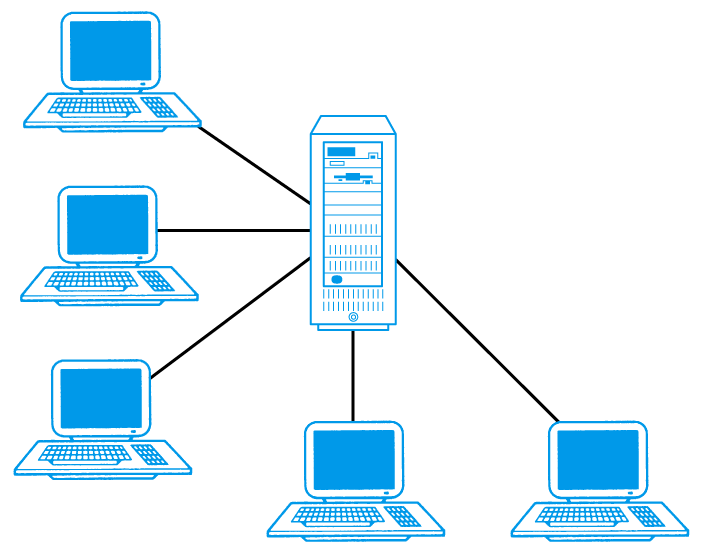
\includegraphics[width=.9\linewidth]{img/Teleprocessing.png}
  \caption{Teleprocessing}
  \label{fig:Teleprocessing}
\end{subfigure}
\begin{subfigure}{.49\textwidth}
  \centering
  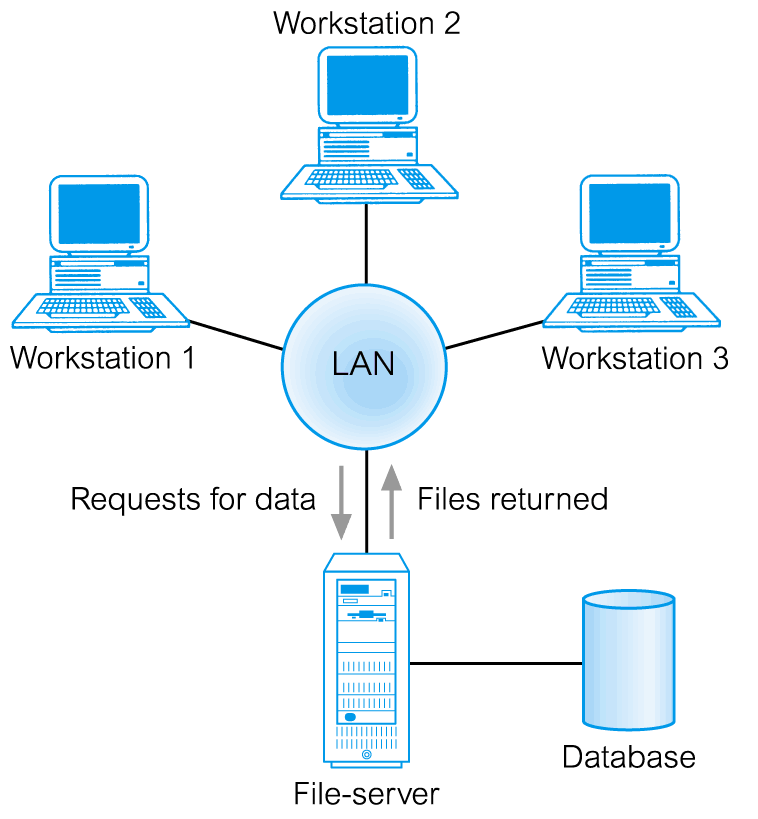
\includegraphics[width=.9\linewidth]{img/FileServer.png}
  \caption{File-Server}
  \label{fig:FileServer}
\end{subfigure}
\begin{subfigure}{.49\textwidth}
  \centering
  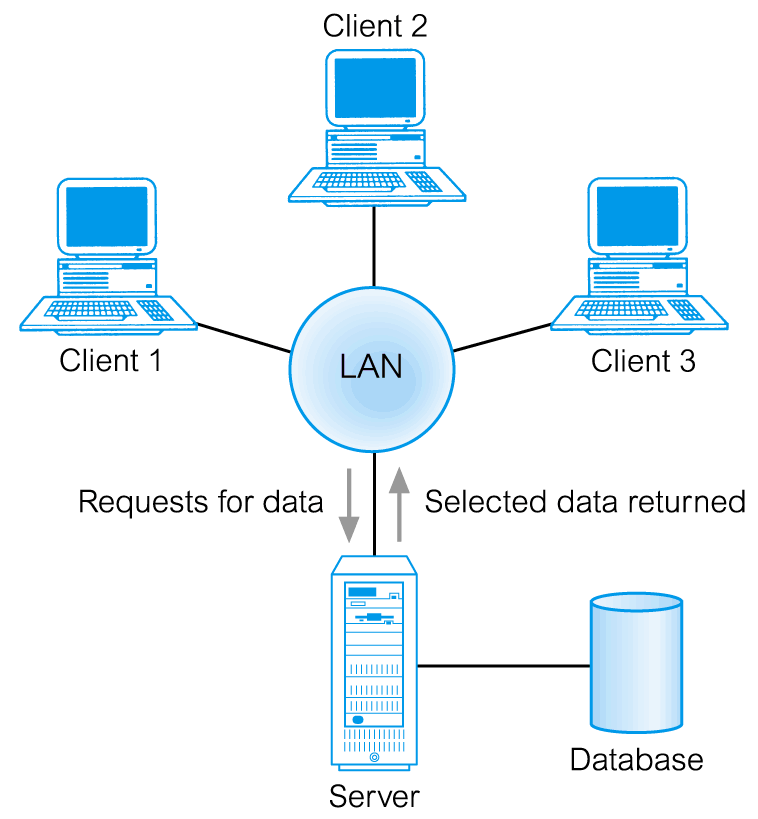
\includegraphics[width=.9\linewidth]{img/Tier2Server.png}
  \caption{2-tier client-server}
  \label{fig:Tier2Server}
\end{subfigure}
\begin{subfigure}{.49\textwidth}
  \centering
  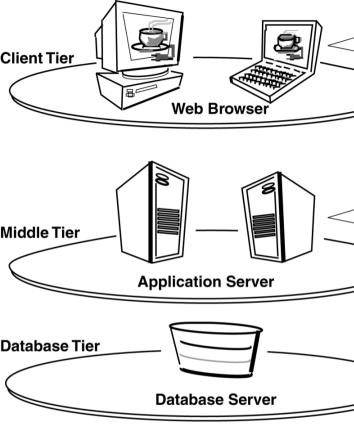
\includegraphics[width=.9\linewidth]{img/Tier3Server.png}
  \caption{3-tier client-server}
  \label{fig:Tier3Server}
\end{subfigure}
\caption{Verschillende harware-architecturen}
\label{fig:HardwareArchitecturen}
\end{figure}

\subsection{Middleware}
Middleware is software die softwarecomponenten of applicaties verbindt.
Dit is nodig wanner gedistribueerde systemen te complex worden zonder een gemeenschappelijke interface.

$\Rightarrow$ Doel: verbergen van onderliggende complexiteit van gedistribueerde systemen.

\subsubsection{Asynchrone Remote Procedure Call}
Bij asynchrone RCP stuurt de client een verzoek naar de server zonder te wachten op antwoord.
Als de connectie verbroken wordt dan moet de client opnieuw beginnen.

$\Rightarrow$ Gebruiken indien integriteit niet belangrijk is.

Er zijn zes types middleware:
\begin{enumerate}
\item Asynchrone RPC
\item Synchrone RPC
\item Publish/Subscribe
\item Message oriented middleware
\item Object Request Broker
\item SQL-oriented data acces
\end{enumerate}
\subsubsection{Synchrone Remote Procedure Call}
Bij synchrone RCP stuurt de client een verzoek naar de server wacht op antwoord.
Zolang de server bezig is met het verzoek is de client geblokkeerd.

$\Rightarrow$ Gebruiken indien integriteit uiterst belangrijk is.

\subsubsection{Publish/Subscribe}
Publish/Subscribe is een asynchroon messaging protocal.
De clients zijn abonnees en kunnen zich inschrijven om boodschappen van publishers te ontvangen.

Boodschappen zijn gecatalogeerd in klassen en een abonnee kan zich inschrijven in één of meerdere klassen.

\subsubsection{Message Oriented Middleware}
Bij MOM staat de software zowel op de client als op de server.

Er gebeuren asynchrone calls tussen client- en server-applicaties.

Er is een wachtrij die dient als tijdelijke opslag indien de bestemming bezet of niet geconnecteerd is.

\subsubsection{Object Request Broker}
Bij ORB is er communicatie en data-uitwisseling tussen objecten.

Common ORB Architecture (CORBA) is een standaard om software componenten, geschreven in verschillende talen en draaied op verschillende computers, met elkaat te laten communiceren.

\subsubsection{SQL-oriented data access}
SQL-oriented data access verbint applicaties met een database over het net.
Het vertaalt SQL requests naar de eigen SQL van de database.

\subsubsection{Middleware voor transactiebeheer}
\textbf{Transaction Processing Monitor}

Complexe applicaties zijn vaak gebouwd op verschillende resource managers.

TP Monitor controleert het dataverkeer tussen clients en servers.

TP Monitor is een middleware component die toegang geeft tot de diensten van een aantal resource managers en zorgt voor een uniforme interface voor programmeurs die transactionele software ontwikkelen.

Er is een verhoogde \textit{schaalbaarheid} door transaction routing.

Er is \textit{taaklastbeheersing} want de TP monitor kan zien welke server het minst belast is en daar de client-calls naar toe dirigeren.

Er zijn \textit{hetrogene bronnen} mogelijk.

Er is \textit{funneling}: niet alle clients moeten constant online zijn
$\rightarrow$ TP monitor kan user requests sturen naar reeds openstaande connecties.

Kortweg kan gezegd worden dat de TP monitor een transaction manager is.

\subsection{Webservices}
Een webservice is een software systeem, dat ontworpen werd voor interactie tussen applicaties en webservers.

Webservices delen business logica, dataen processen m.b.v. een programmeerbare interface over een netwerk.

Ontwikkelaars voegen de webservice toe aan een webpagina om specifieke functionaliteit aan te bieden aan de gebruikers.

Webservices gebruiker algemeen aanvaarde technologieën en standaarden zoals: XML, SOAP, WSDL en UDDI.

\subsection{Service-Oriented Architecturen}
Business-georiënteerde software-architectuur voor het bouwen van applicaties en business processen implementeren als een set van gepubliceerde services.

Granulariteit moet relevant zijn voor de service-gebruiker.

Services kunnen aangeroepen, gepubliceerd en gevonden worden op een abstracte manier, d.w.z. los van de implementatiedetails, maar gebaseerd op een unieke standaar-interface.

Laat toe dat applicaties zich snel kunnen aanpassen aan wijzigende business-processen t.g.v. bijvoorbeeld gewijzigde marktomstandigheden.

\subsection{Cloud Computing}
\subsubsection{Kenmerken}
\textbf{On-demand self-service}: Gebruikers kunnen clouddiensten verkrijgen, configureren en deployen zonder hulp van een provider.

\textbf{Broad network acces}: Toegankelijk van overal, vanaf elke standaardplatform.

\textbf{Resource pooling}: Computer resources van provider zitten in een pool, die meerdere gebruikers bedient.
Fysieke en virtuele resources worden dynamisch toegekend volgens de behoefte van een gebruiker op een bepaald moment.

\textbf{Snelle elasticiteit}: Piekbehoeften van de klant worden opgevangen door pooling.
Er is een sterk verminderd risico op uitval en onderbrekingen van de dienstverlening.
Toekenning van de capaciteit kan geautomatiseerd gebeuren op basis van vraag $\rightarrow$ \textit{scalability}.

\textbf{Metingen van afgenomen diensten}: Provider meet gebruik van storage, CPU, bandbreedte\dots
Deze metingen worden dan gebruik voor de Service Level Agrements (SLA) en de facturatie.

\subsubsection{Software as a Service}
Bij SaaS bevinden zich software en data in de cloud.
De toegang wordt verzorgt via een thin client (bv. web browser).
De gebruiker kan hier beperkte toegang hebben tot configuratie-instellingen.

\subsubsection{Platform as a Service}
Bij PaaS bouwt de klant de webapplicatie zonder aankoop/onderhoud van software en infrastuctuur.
De provider beheert de infrastructuur (netwerk, OS en storage).
De klant beheert het deployment en de configuratie van applicaties.

\subsubsection{Infrastructure as a Service}
Bij SaaS levert de provider servers, storage, netwerk en OS aan de gebruikers, gebundeld al on-demand service.
Dit model wordt typisch gebruikt voor platform-virtualisatie.
De facturatie gebeurt volgens gebruik.

\begin{figure}[H]
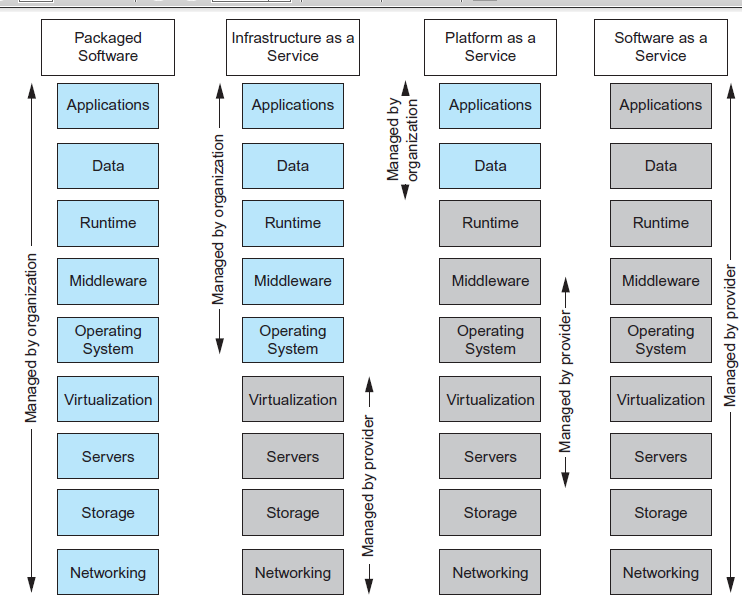
\includegraphics[scale=1]{./img/VergelijkingServiceModellen}
\caption{Vergelijking van service-modellen}
\label{fig:VergelijkingServiceModellen}
\end{figure}

\subsubsection{Voordelen van cloud computing}
\textbf{Kostenreductie}: vermijd kapitaalintensieve investeringen voor opbrengsten.

\textbf{Scalability}: bijkomende resources schaf je aan volgens behoefte.

\textbf{Security en betrouwbaarheid}: providers kunnen expertise en resources verdelen over meerdere klanten.
Een individuele klant kan dit niet betalen.

\textbf{Toegang tot nieuwste technologieën}: systemen moeten niet meer afgeschreven zijn om nieuwe technologieën te kunnen gebruiken, want je huurt de systemen.

\textbf{Snellere ontwikkeling}: platform van de provider zorgt voor software en diensten die ontwikkelingscyclus kunnen versnellen.

\textbf{Prototyping/Load testing op grote schaal}: de provider heeft hiervoor de resources.

\textbf{Verhoogde competitiviteit}: organisaties kunnen focussen op hun kerncompetenties i.p.v. op IT-infrastructuren.

\textbf{Flexibeler werken} : bv. toegang via mobile devices.

\subsubsection{Risico's van cloud computing}
\textbf{Afhankelijkheid van het netwerk}: Stroomonderbrekingen, bandbreedte-problemen en onderbreking dienstverlening.

\textbf{Afhankelijkheid van de systemen}: je vertrouwt op beschikbaarheid en betrouwbaarheid van systemen van de provider.

\textbf{Afhankelijkheid van de cloud provider}: deze kan failliet gaan of overgenomen worden door concurrent met mogelijk onmiddelijke stopzetting van de service.

\textbf{Gebrek aan controle}: je beslist niet zelf over bv. backup-policy.

\textbf{Gebrek aan transparantie over achterliggende verwerking}

\subsection{Cloud gebaseerde databanken}
Cloud gebaseerde databanken zijn een voorbeel van SaaS.
Er zijn twee basiscategorieën:
\begin{enumerate}
\item Data as a Service (DaaS)
\item Database as a Service (DBaaS)
\end{enumerate}
Het verschil tussen beiden zit hoofdzakelijk in hoe de data beheerd wordt.

\subsubsection{Database as a Service}
DBaaS biedt een volledige databankfunctionaliteit aan ontwikkelaars. Dit model voorziet ook in een management-laag, die continue monitoring en cofiguratie van de databank toelaat:
\begin{itemize}
\item geoptimaliseerde scalability
\item hoge beschikbaarheid
\item multi-tenancy: meerdere client-organisaites worden gelijktijdig bediend.
\item effectief reource management in de cloud $\rightarrow$ ontwikkelaar moet zich niet bezighouden met dba-taken.
\end{itemize}

\subsubsection{Data as a Service}
Bij DaaS zit de data-definitie en querying in de cloud.

DaaS implementeert geen typische DMBS-interface (bv SQL), maar de data is beschikbaar via API's. $\rightarrow$ verhoogde controle door de provider.

DaaS laat toe om je data aan anderen ter beschikking te stellen.

\subsection{Mobile Databases}
Mobile databases dienen om data persistent te maken.
Hierbij zijn er twee mogelijkheden waarbij de keuze gemaakt wordt door de app developer.
\begin{enumerate}
\item Database op afstand die verbonden wordt met het mobiele toestel (internet nodig).
\item Database die opgeslagen wordt op het mobiele toestel (offline gebruik mogelijk).
\end{enumerate}

Vaak wordt met een middle tier zoals een mobile web service gewerkt.
Hierbij is er geen rechtstreeks contact tussen de client en de databank.

De client stuurt een HTTP request naar de webservice.
De client kan vaak in zijn request naar de webservice kiezen hoe hij de data wil ontvangen (=content negotiation).
De webservice communiceert met de databank en haalt de data binnen.
Naar gelang wat werd gevraagd, zal de web service de resultset omzetten.
Dit resultaat wordt dan aangeboden aan de client.
Op die manier is er nooit rechtstreeks contact tussen de databank en de client.

\subsubsection{Voordelen}
Er is nooit rechtstreeks contact tussen de client en de DB.

Clients kunnen kiezen in welk formaat ze de data wensen te ontvangen.

Schaalbaarheid hangt niet enkel af van de databank maar ook van de webservice $\rightarrow$ wordt verdeeld.

Dezelfde web service (logica) kan gebruikt worden door verschillende clients/platformen $\rightarrow$ reuse.

Request kan over https gebeuren $\rightarrow$ veiligheid.

\subsubsection{Nadelen}
Performantie wordt o.a. bepaald door de internetverbinding.

Behalve een DB Server ook nog nood aan eene extra technologie voor de middle tier.

Er is steeds internetverbinding nodig.

\subsubsection{Mobile database lokaal}
De lokale mobile database wordt ook wel de offline storage genoemd.

De DB is platform afhankelijk, maar is wel relatief snel.

De DB neemt opslagplaats in op het device.
Hierdoor is de app zelf verantwoordelijk voor het updaten van de data.

\section{Database ontwerp - DDL}
\subsection{Database}
\subsubsection{Een database creëren}
Bij creatie van een DB worden fysiek 2 files gemaakt: een datafile (mdf) en een logfile (ldf).
Er kunnen meerdere datafiles zijn, nl. de secondary data files (ndf).
Er kunnen ook meerdere logfiles zijn.

Bij creatie van een DB wordt een kopie genomen van de model database, deze bevat systeemtabellen en systeemviews.

\begin{figure}[H]
\centering
  	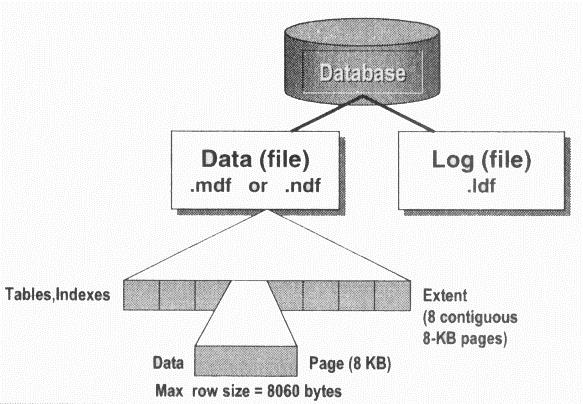
\includegraphics[width=.5\linewidth]{img/DatabaseCreatie.png}
  	\caption{Opbouw van een database}
  	\label{fig:DatabaseCreatie}
\end{figure}

Data wordt opgeslagen in blokken van 8 KB aaneensluitende diskspace, dit noemt met een pagina.
Eén rij kan niet op meerdere pagina’s bewaard worden, een rij mag maximaal 8060 b groot zijn (8KB – ruimte overhead).
8 opeenvolgende pagina’s worden 1 extend (64 KB).
Een tabel, index wordt opgeslagen in een extend.
Dit alles is te zien op figuur~\ref{fig:DatabaseCreatie}

Logfiles bevatten informatie nodig voor recovery.
De logfile-grootte is per default 25\% van grootte van de datafile.

In sql creëert men een database als volgt:
\begin{lstlisting}[language=sql]
CREATE DATABASE database_name
\end{lstlisting}

Men kan hierbij ook parameters meegeven:
\begin{lstlisting}[language=sql, breaklines=true]
CREATE DATABASE oefenDB 
ON PRIMARY(
	NAME = oefenDB_data,
	FILENAME = 'C:\Program Files\Microsoft SQL Server\ MSSQL.1\MSSQL\Data\oefenDB.mdf',
	SIZE = 10MB, MAXSIZE = 15MB, FILEGROWTH = 20%)
LOG ON (
	NAME = tttoefenDB_log,
	FILENAME = 'C:\Program Files\Microsoft SQL Server\ MSSQL.1\MSSQL\Data\oefenDB.ldf',
	SIZE = 3MB, MAXSIZE = 5MB, FILEGROWTH = 1MB)
\end{lstlisting}

\subsubsection{Een database verwijderen}
\begin{lstlisting}[language=sql, breaklines=true]
DROP DATABASE database_name
\end{lstlisting}

Hierbij dient opgemerkt te worden dat de systeem databank niet verwijderd kan worden.

\subsubsection{Een database wijzigen}
\begin{itemize}
\item beheer van de groei van de database en log file
\item uitbreiden/verminderen van grootte van database en log
\item toevoegen/verwijderen van secondary database files, log files
\end{itemize}

Wijzigen van de groote van het logbestand:
\begin{lstlisting}[language=sql, breaklines=true]
ALTER DATABASE oefenDB
MODIFY FILE (name = 'oefenDB_log', size = 10MB)
\end{lstlisting}

Toevoegen van een databastand:
\begin{lstlisting}[language=sql, breaklines=true]
ALTER DATABASE oefenDB
ADD FILE (
	name = oefenDB2,
	filename = 'C:\Program Files\Microsoft SQL Server\ MSSQL.1\MSSQL\Data\oefenDB2.ndf',
	size = 10MB,
	maxsize = 15MB)
\end{lstlisting}

\subsection{Tabellen}
\subsubsection{Een tabel creëren}
Bij de creatie van een tabel specifieren we:
\begin{itemize}
\item de naam van de tabel.
\item de definitie van de kolommen (naam, datatype \dots).
\item definitie van de constraints.
\end{itemize}

\begin{lstlisting}[language=sql, breaklines=true]
CREATE TABLE student(
	studentno int NOT NULL,
	lastname varchar(30) NOT NULL,
	firstname varchar(30) NOT NULL,
	gender char(1) NOT NULL,
	photograph image NULL)
\end{lstlisting}

\subsubsection{Een tabel wijzigen}
Mogelijke wijzigingen aan een tabel omvatten:
\begin{itemize}
\item toevoegen van kolommen.
\item wijzigen van kolommen.
\item verwijderen van kolommen.
\end{itemize}

\begin{lstlisting}[language=sql, breaklines=true]
ALTER TABLE student(
	ADD address varchar(40) NULL,
	ALTER COLUMN address varchar(50) NULL,
	DROP COLUMN address)
\end{lstlisting}

\subsubsection{Een tabel verwijderen}
Bij het verwijderen van een tabel diet men rekening te houden met de afhankelijkheden.

\begin{lstlisting}[language=sql, breaklines=true]
DROP TABLE student
\end{lstlisting}

\subsection{Contraints}
\subsubsection{Identity waarden}
Een identity kolom bevat voor elke rij een unieke waarde, die sequentieel door het systeem gegenereerd wordt.
Er is slechts één identity kolom per tabel mogelijk.
De identity kolom kan niet NULL zijn en kan niet door gebruikers aangepast worden.

\begin{lstlisting}[language=sql, breaklines=true]
CREATE TABLE studentVoorbeeldIdentity(
	studentno int identity(100, 5) NOT NULL,
	lastname varchar(30) NOT NULL,
	firstname varchar(30) NOT NULL,
	gender char(1) NOT NULL,
	photograph image NULL)
\end{lstlisting}

\subsubsection{Data integriteit}
Soorten:
\begin{itemize}
\item domein integriteit
\item entity integriteit
\item referentiële integriteit
\end{itemize}

\subsubsection{Definitie van constraints}
Via create table en als onderdeel van de kolomdefinitie:
\begin{lstlisting}[language=sql, breaklines=true]
CREATE TABLE studentVoorbeeldIdentity(
	studentno int NOT NULL unique)
\end{lstlisting}

Via alter table en als aparte lijn:
\begin{lstlisting}[language=sql, breaklines=true]
ALTER TABLE studentVoorbeeldIdentity(
	CONSTRAINT studentno_U unique(studentno)
\end{lstlisting}

Zowel bij creatie al bij wijzigen kan gekozen worden voor onderdeel van de kolomdefinitie als voor aparte lijn.
NULL en DEFAULT constraints kunnen enkel bij definitie van de kolom worden opgegeven.

\subsubsection{Check constraint}
\begin{lstlisting}[language=sql, breaklines=true]
gender char(1) default 'M' check(gender in ('M','F')) not null
\end{lstlisting}

\subsubsection{Primary key constraint}
\begin{lstlisting}[language=sql, breaklines=true]
studentno int primary key
\end{lstlisting}

of

\begin{lstlisting}[language=sql, breaklines=true]
constraint studentno_PK primary key(studentno)
\end{lstlisting}

\subsubsection{Foreign key constraint}
De foreign key wordt gebruikt om verbanden tussen relaties uit te drukken. NULL waarden zijn niet toegelaten.
\begin{lstlisting}[language=sql, breaklines=true]
constraint class_fk foreign key(class) references class(classID)
\end{lstlisting}
De foreign key legt ook de trapsgewijze (cascading) referentiële integriteitsacties vast.

\subsection{Views}
\subsubsection{Introductie}
Een view is een SELECT statement die onder een eigen naam wordt bewaard.
Een view is bijgevolg een soort virtuele tabel samengesteld uit andere tabellen of views.

De voordelen hiervan zijn dat de complexiteit van de database verborgen is.
Gebruikers krijgen functionaliteit en rechten op maat.
Views vereenvoudigen de beveiliging van de database.
Data wordt ook georganiseerd voor de export naar andere applicaties.

\begin{lstlisting}[language=sql, breaklines=true]
CREATE VIEW view_name [(column_list)]
AS select_statement
\end{lstlisting}

Views kunnen net als tabellen verwijders en gewijzigd worden.

\subsection{Indexen en performatie}
De heap is een ongeordende verzameling van data-pages zonder clustered index. Dit is de standaard opslag van een tabel.

Een index is een geordende structuur die op de records uit een tabel wordt gelegd.
Deze zijn snel toegankelijk dankzij een boomstructuur.
Dankzij indices kan de toegang tot data versnelt worden en kan uniciteit van de rijen afgedwongen worden.
Daarentegen nemen indexen veel opslagruimte in beslag en ze kunnen de performantie ook doen dalen.

\subsubsection{Clustered Index}
De fysische volgorde van de rijen in een tabel is deze van de clustered index.
Elke tabel kan maar één clustered index hebben.

De voordelen t.o.v. table scan zijn dat  een dubbel gelinkte lijst zorgt voor de volgorde bij het lezen van sequentiële records.
Er zijn ook geen forward pointers.
De clustered index legt unieke waarden op.

\begin{figure}[H]
\centering
  	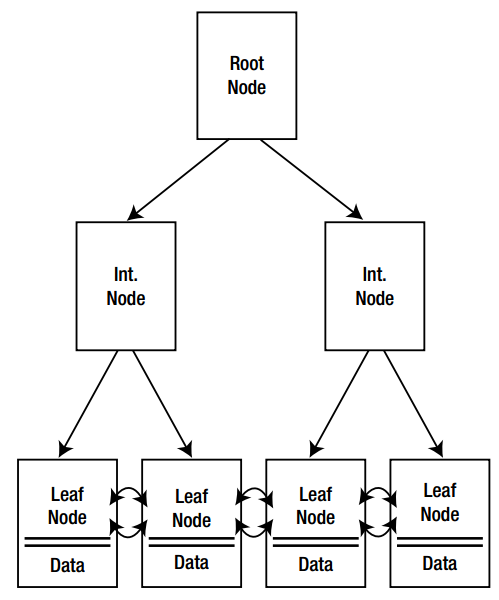
\includegraphics[width=.35\linewidth]{img/ClusteredIndex.png}
  	\caption{Clustered index}
  	\label{fig:ClusteredIndex}
\end{figure}

\subsubsection{Non-clustered Index}
De non-clustered index is de default index, deze werkt trager dan de clustered index.
Wel zijn er meerdere non clustered indexen mogelijk per tabel.
Elke leaf bevat een sleutelwaarde en een row locator, deze wijst naar de positie in de clustered index als die bestaat, anders naar de heap.

\begin{figure}[H]
\centering
  	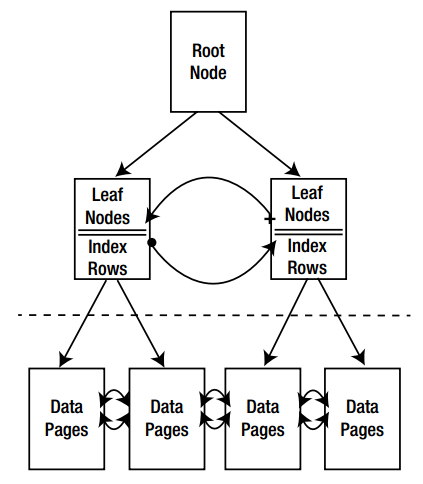
\includegraphics[width=.35\linewidth]{img/NonClusteredIndex.png}
  	\caption{Non-clustered index}
  	\label{fig:NonClusteredIndex}
\end{figure}

\subsubsection{Covering index}
Als een non-clustered indec een query niet volledig covert, dan moet de databank voor elke rij een lookup doen om de data op te halen.
Een covering index is in wezen een non-clustered index die alle kolommen bevat die nodig zijn voor een bepaalde query.

\subsubsection{Operaties op een index}
Creatie:
\begin{lstlisting}[language=sql, breaklines=true]
CREATE [UNIQUE] [CLUSTERED | NONCLUSTERED]
	INDEX index_naamON tabel(kolom[,...n])
\end{lstlisting}

Verwijderen:
\begin{lstlisting}[language=sql, breaklines=true]
DROP INDEX table_name.index_name[,...n]
\end{lstlisting}

\section{Postrelationele DBMS}
\subsection{SQL als volwaardige taal}
Procedurele uitbreidingen op SQL zijn merkgebonden. Database systemen die gebruik maken van deze uitbreidingen zijn dus moeilijker om te zetten van één RDBMS op een andere.

In het vervolg van deze samenvatting gaan we verder met t-SQL, die gebruikt wordt bij SQL Server.

De meeste database systemen voorzien al een aantal standaard SQl functies zoals minimum, maximum, som, gemiddelde, aantal \dots

SQL Server heeft nog een aantal extra functies zoals datediff, substring, len, round \dots

Naast deze functies is het ook nog mogelijk om user defined functies aan te maken.

\subsubsection{Voordelen van PSM}
\begin{itemize}
\item Code modularisatie
	\begin{itemize}
	\item reduceren redundante code: veel gebruikte queries in Stored Procedures en hergebruiken in 3GL.
	\item vaak voor de CRUD-operaties
	\item minder onderhoud bij schema-wijzigingen
	\end{itemize}
\item Security
	\begin{itemize}
	\item rechtstreekse queries op tabellen zijn uitgesloten
	\item via stored procedures vastleggen wat kan en wat niet
	\item vermijd SQL-injection, door gebruik input-parameters
	\end{itemize}
\item Centrale administratie van (delen van) DB-code.
\end{itemize}

\subsubsection{Nadelen van PSM}
\begin{itemize}
\item Beperkte schaalbaarheid
\item Vendor lock-in
	\begin{itemize}
	\item Er is geen standaard syntax
	\end{itemize}
\item Twee programmeertalen
\item Twee debugomgevingen
\item Beperkte OO-ondersteuning
\end{itemize}

\subsubsection{Vuistregels}
\begin{itemize}
\item Vermijd PSM voor grotere business logica
\item Gebruik PSM voor technische zaken: logging, auditing, validatie
\item Maak keuze voor portabiliteit/vendor lock-in in overleg met de business of corporate IT policies.
\end{itemize}

\subsubsection{Stored procedure}
Een stored procedure is een benoemde verzameling sql en control-of-flow opdrachten (programma) die opgeslagen wordt als een database object.
De stored procedure is analoog aan procedures uit andere talen.
Het kan aangeroepen worden vanuit een programma, trigger of stored procedure.

\subsection{Variabelen}
\subsubsection{Lokale variabelen}
\begin{lstlisting}[language=sql, breaklines=true]
DECLARE @lname varchar(40), @rijtelling int
SET @lname = 'Ringer'
SELECT @rijtelling = count(*)
FROM Authors
Where au_lname = @lname
PRINT 'Aantal werknemers met naam ' + @lname + ' = ' + str(@rijtelling)
\end{lstlisting}
Merk bij bovenstaande code op dat de naam van een variabele steeds wordt voorafgegaan door @.
Het toekennen van een waarde gebeurt via SET of SELECT

\subsubsection{Control flow met Transact SQL}
In een programma kan je het verloop bepalen via o.a.:
\begin{itemize}
\item Instructie niveau
	\begin{itemize}
	\item BEGIN ... END
	\item IF ... ELSE
	\item WHILE ...
		\begin{itemize}
		\item BREAK
		\item CONTINUE
		\end{itemize}
	\item RETURN
	\end{itemize}
\item Rij niveau
	\begin{itemize}
	\item CASE ... END
	\end{itemize}
\end{itemize}

\subsubsection{Gebruik van commentaar}
\begin{itemize}
\item Inline commentaar
	\begin{itemize}
	\item --commentaar
	\end{itemize}
\item Block commentaar
	\begin{itemize}
	\item /*commentaar*/
	\end{itemize}
\end{itemize}

\subsection{Cursors}
SQL statements werken standaar met een complete resultaatset en niet met individuele rijen. Cursors laten toe om met individuele rijen te werken.
Een cursor is dus een database object die wijst naar een resultaatset. Via de cursor kan men aangeven met wlke rij uit de resultaatset men wenst te werken.

\subsubsection{Declaratie van een cursor}
\begin{lstlisting}[language=sql, breaklines=true]
DECLARE <cursor_name> [INSENSITIVE][SCROLL] CURSOR FOR
<SELECT_statement>
[FOR {READ ONLY | UPDATE[OF <column list>]}]
\end{lstlisting}

\begin{itemize}
\item INSENSITIVE
	\begin{itemize}
	\item de cursor werkt met een tijdelijke kopie van de gegevens
		\begin{itemize}
		\item wijzigingen in onderliggende tabellen worden niet gereflecteerd in gegevens opgehaald via de cursor.
		\item de cursor kan niet gebruikt worden om tabellen te wijzigen
		\end{itemize}
	\item wanneer INSENSITIVE weggelaten wordt dan worden deletes en updates wel degelijk gereflecteerd in de cursor. 
	
	Dit is wel minder performant aangezien elke fetch nu resulteert in en nieuwe select opdracht.
	\end{itemize}
\item SCROLL
	\begin{itemize}
	\item alle soorten fetch operaties zijn bruikbaar
		\begin{itemize}
		\item FIRST, LAST, PRIOR, NEXT, RELATIVE en ABSOLUTE
		\end{itemize}
	\item wanneer SCROLL weggelaten wordt dan kan je enkel via NEXT data ophalen.
	\end{itemize}
\item READ ONLY
	\begin{itemize}
	\item verhindert dat je via de cursor de onderliggende tabellen kan wijzigen
	\item per default kan je via de cursor wel de onderliggende tabellen aanpassen
	\end{itemize}
\item UPDATE
	\begin{itemize}
	\item benoemen van specifieke kolommen die kunnen gewijzigd worden via de cursor.
	
	Enkel kolommen benoemd in deze clause kunnen gewijzigd worden.
	\end{itemize}
\end{itemize}

\subsubsection{Openen van een cursor}
\begin{lstlisting}[language=sql, breaklines=true]
OPEN <cursor name>
\end{lstlisting}

Hiermee wordt de cursor geopend en vervolgens opgevult met het SELECT statement dat in de declaratie was meegegeven.

De cursors current row pointer wordt gepositioneerd net voor de eerste rij in de actieve set.

\subsubsection{Data ophalen via een cursor}
\begin{lstlisting}[language=sql, breaklines=true]
FETCH[NEXT | PRIOR | FIRST | LAST | {ABSOLUTE|RELATIVE <rownumber>}]
FROM <cursor name>
[INTO <variable name> [,...<last variable name>]]
\end{lstlisting}
\begin{itemize}
\item De cursor wordt gepositioneerd
	\begin{itemize}
	\item op de "volgende" (of vorige, eerste, laatste\dots) rij
	\item per default wordt gepositioneerd via NEXT, voor andere manieren moet je een SCROLL-able cursor gebruiken.
	\end{itemize}
\item De gegevens worden opgehaald
	\begin{itemize}
	\item zonder INTO clause worden resulterende gegevens op het scherm getoond.
	\item met INTO clause worden gegevens in de opgegeven variabelen gestopt. Hierbij moet men opletten dat de variabelen gedeclareerd zijn.
	\end{itemize}
\end{itemize}

Een voorbeeld:
\begin{lstlisting}[language=sql, breaklines=true]
DECLARE @au_lname varchar(40), @au_fname varchar(20)
FETCH NEXT FROM authors_cursor
INTO @au_lname, @au_fname
WHILE @@FETCH_STATUS = 0 BEGIN
	PRINT 'Author: ' + @au_fname + ' ' + @au_lname
	FETCH NEXT FROM authors_cursor
	INTO @au_lname, @au_fname
END
\end{lstlisting}

\subsubsection{Sluiten van een cursor}
\begin{lstlisting}[language=sql, breaklines=true]
CLOSE <cursor_name>
\end{lstlisting}

\begin{itemize}
\item de cursor wordt gesloten
	\begin{itemize}
	\item de definitie van de cursor blijft bestaan
		\begin{itemize}
		\item er mogelijkheid om de cursor te heropenen
		\end{itemize}
	\end{itemize}
\end{itemize}

\subsubsection{Dealloceren van een cursor}
\begin{lstlisting}[language=sql, breaklines=true]
DEALLOCATE <cursor_name>
\end{lstlisting}


\begin{itemize}
\item de cursordefinitie wordt verwijderd
	\begin{itemize}
	\item wanneer dit de laatste referentie naar de cursor was dan worden alle resources voor die cursor vrijgegeven
	\item indien de cursor nog niet gesloten is da deallocate de cursor automatisch sluiten
		\begin{itemize}
		\item een close opdracht net voor een deallocatie opdracht hoeft dus niet
		\end{itemize}
	\end{itemize}
\end{itemize}

\subsubsection{Updaten via een cursor}
\begin{lstlisting}[language=sql, breaklines=true]
UPDATE <table name>
SET ...
WHERE CURRENT OF <cursor name>
\end{lstlisting}

\subsubsection{Verwijderen via een cursor}
\begin{lstlisting}[language=sql, breaklines=true]
DELETE FROM <table name>
WHERE CURRENT OF <cursor name>
\end{lstlisting}

\subsection{Stored Procedures}
\subsubsection{Creatie van een SP}
\begin{lstlisting}[language=sql, breaklines=true]
CREATE PROCEDURE <proc_name> [parameter declaratie]
AS
<sql_statements>
\end{lstlisting}
\begin{itemize}
\item aanmaken db-object: via DDL instructie
\item controle op syntax
	\begin{itemize}
	\item enkel indien syntactisch correct wordt de stored procedure opgeslaan in de catalogus.
	\end{itemize}
\end{itemize}

\subsubsection{Wijzigen van een SP}
\begin{lstlisting}[language=sql, breaklines=true]
ALTER PROCEDURE <proc_name> [parameter declaratie]
AS
<sql_statements>
\end{lstlisting}

\subsubsection{Verwijderen van een SP}
\begin{lstlisting}[language=sql, breaklines=true]
DROP PROCEDURE <proc_name>
\end{lstlisting}

\subsubsection{Uitvoeren van een SP}
\begin{lstlisting}[language=sql, breaklines=true]
EXCUTE <proc_name> [parameters]
\end{lstlisting}

\begin{itemize}
\item bij eerste uitvoering
	\begin{itemize}
	\item compilatie en optimalisatie
	\end{itemize}
\item hercompilatie forceren
	\begin{itemize}
	\item wenselijk bij wijzigingen aan structuur databank
	\begin{lstlisting}[language=sql, breaklines=true]
	execute uspOrdersSelectAll with recompile
	\end{lstlisting}
	\begin{lstlisting}[language=sql, breaklines=true]
	execute sp_recompile uspOrdersSelectAll
	\end{lstlisting}
	\end{itemize}
\end{itemize}

\subsubsection{De returnwaarde van een SP}
\begin{itemize}
\item Bij uitvoering keert een SP een returnwaarde terug
	\begin{itemize}
	\item deze waarde is een int
	\item de default return waarde is 0.
	\end{itemize}
\item return statement
	\begin{itemize}
	\item uitvoering van de SP wordt gestopt
	\item laat toe om de returnwaarde te bepalen
	\end{itemize}
\end{itemize}

Creatie van een SP met expliciete returnwaarde:
\begin{lstlisting}[language=sql, breaklines=true]
CREATE PROCEDURE usp_OrdersSelectAllAS
select * from orders
return @@ROWCOUNT
\end{lstlisting}

Gebruik van een SP met een returnwaarde:
\begin{lstlisting}[language=sql, breaklines=true]
DECLARE @returnCode int
EXEC @returnCode = usp_OrdersSelectAll
PRINT 'Er zijn ' + str(@returnCode) + ' records.'
\end{lstlisting}

\subsubsection{SP met parameters}
Via een input parameter kan men een waarde doorgeven aan de SP.

Via een output parameter kan men eventueel een waarde doorgeven aan de SP en krijgt men een waarde terug van de SP.

\begin{lstlisting}[language=sql, breaklines=true]
CREATE PROCEDURE usp_OrdersSelectAllForCustomer
@customerIDnchar(5) = 'ALFKI',
@count intOUTPUT
AS
SELECT @count = count(*)
FROM orders WHERE customerID= @customerID
\end{lstlisting}
Merk op dat 'ALFKI' een default waarde is die ingesteld wordt.

\begin{itemize}
\item aanroepen van de SP
	\begin{itemize}
	\item voorzie steeds het keyword OUTPUT voor output parameters
	\item twee manieren om actuele parameters door te geven
		\begin{itemize}
		\item gebruik formele parameternaam
		\item positioneel
		\end{itemize}
	\end{itemize}
\end{itemize}

Parameters via formele naam doorgeven:
\begin{lstlisting}[language=sql, breaklines=true]
DECLARE @aantal int
EXECUTE usp_OrdersSelectAllForCustomer
@customerID= 'ALFKI',
@count= @aantal OUTPUT
PRINT @aantal
\end{lstlisting}

Parameters positioneel doorgeven:
\begin{lstlisting}[language=sql, breaklines=true]
DECLARE @aantalint
EXEC usp_OrdersSelectAllForCustomer'ALFKI', @aantalOUTPUT
PRINT @aantal
\end{lstlisting}

\subsubsection{Error handling}
@@erroris een systeemfunctie die het foutnummer bevat van de laatst uitgevoerde opdracht. De waarde 0 wijst op succesvolle uitvoering.

Alle foutboodschappen zitten in de systeemtabel sysmessages.
\begin{lstlisting}[language=sql, breaklines=true]
SELECT * FROM master.dbo.sysmessages
WHERE error = @@ERROR
\end{lstlisting}
Eigen fouten kan men genereren via raiseerror(msg,severity,state)

\subsection{Triggers}
Trigger is gekoppeld aan een database actie.
\subsubsection{Procedurele database objecten}
\begin{table}[H]
\centering
\begin{tabular}{|c|c|c|p{2cm}|p{3cm}|}
\hline
Soort & Batches & Opgeslaan als & Uitvoering & Ondersteunt\newline parameters\\
\hline
Script & meerdere & Apart bestand & Client tool & nee\\
\hline
Stored Procedure & 1 & Database Object & Applicatie of SQL & ja\\
\hline
User defined function & 1 & Database Object & Applicatie of SQL & ja\\
\hline
Trigger & 1 & Database Object & DML, DDL, login-logoff statement & nee\\
\hline
\end{tabular}
\caption{Procedurele programma's}
\label{tab:procedurele_programmas}
\end{table}
Een batch is een programma zonder interactie.

\subsubsection{Definitie}
Een trigger is een speciaal type Stored Procedure.

Het is een stuk code dat automatisch uitgevoerd wordt als een neveneffect van een actie op een tabel.

\subsubsection{Gebruik}
\begin{itemize}
\item Validatie van data en complexe constraints
\item Automatische generatie van waarden
\item Ondersteuning voor alerts
\item Bijhouden van audits
\item Replicatie en gecontrolleerd bijhouden van redundante data
\end{itemize}

\subsubsection{Syntax}
\begin{lstlisting}[language=sql, breaklines=true]
CREATE TRIGGER TriggerName
BEFORE | AFTER | INSTEAD OF
INSERT | DELETE | UPDATE [OF TriggerColumnList]

ON TableName
[REFERENCING {OLD | NEW} AS {OldName | NewName}]
[FOR EACH {ROW | STATEMENT}]
[WHEN condition]
<trigger action>
\end{lstlisting}

Trigger Event:
\begin{itemize}
\item bepaalt bij welke gebeurtenis de trigger geactiveerd zal worden.
\item bij update kan eventueel gespecifiëerd worden voor welke kolommen de triggering event gegenereerd wordt.
\end{itemize}

Trigger Condition
\begin{itemize}
\item wanneer de conditie false oplevert wordt er verder niets met de trigger gedaan.
\item wanneer de conditie true oplevert zal de trigger action uitgevoerd worden.
\end{itemize}

Trigger Action:
\begin{itemize}
\item Een aantal SQL-opdrachten
\end{itemize}

Timing:
\begin{itemize}
\item \textbf{Before}: evaluatie van de trigger conditie en eventuele uitvoering van trigger actie gebeurt op de toestand van de DB zoals deze is vóór de triggering event zelf wordt afgehandeld.
\item \textbf{After}: evaluatie van de trigger conditie en eventuele uitvoering van trigger actie gebeurt op de toestand van de DB zoals deze is nadat de triggering event zelf wordt afgehandeld.
\item \textbf{Instead Of}: trigger wordt uitgevoerd ter vervanging van het DML statement.
\end{itemize}

Uitvoering:
\begin{itemize}
\item \textbf{For Each Row}: trigger wordt 'gewekt' voor elk tupel dat wordt gewijzigd door het trigger event.
\item \textbf{For Each Statement}:   1 keer 'gewekt' ongeacht het aantal tupels dat gewijzigd wordt door het trigger event.
\end{itemize}

Verwijzen naar tupels/tabellen in de trigger
\begin{itemize}
\item \textbf{Old/oldName}: in de condition en trigger action kan verwezen worden naar de oude waarden van de tupels.
Dit is niet relevant bij de insert trigger.
\item \textbf{New/newName}: in de condition en trigger action kan verwezen worden naar de nieuwe waarden van de tupels.
Dit is niet relevant bij delete trigger
\end{itemize}

\subsubsection{Uitvoering van een trigger}
Volgorde bij een true-condition:
\begin{enumerate}
\item uitvoering van beforestatement level triggersop de tabel
\item voor elke rij geaffecteerd door de trigger
\begin{enumerate}
\item uitvoering van beforerowlevel triggers
\item uitvoering van de triggering event(i.e. update/delete/insert)
\item toepassen van referentiële constraints
\item uitvoering van afterrowlevel triggers
\end{enumerate}
\item uitvoering van afterstatement level triggersop de tabel
\end{enumerate}

\subsubsection{Voordelen}
Mogelijkheid om functionaliteit in de DB op te slaan en consistent uit te voeren bij elke wijziging aan de DB.

Dus:
\begin{itemize}
\item geen redundante code: functionaliteit op 1 plaats
\item wijzigingen aanbrengen wordt eenvoudig
\item veiligheid: triggers in de database
\item meer processing power
\item past in client-server model
\end{itemize}

\subsubsection{Nadelen}
\begin{itemize}
\item Complexiteit: moeilijk om te debuggen en functionaliteit van applicatie naar DB
\item Verborgen functionaliteit: onverwachte neveneffecten en cascading
\item Performantie: Bij elke wijziging aan de DB moet de trigger conditie geëvalueerd worden.
\item Portabiliteit: Dialect van DBMS
\end{itemize}

\subsubsection{MS SQL Server: Trigger test tabellen}
Er zijn 2 tijdelijke tabellen: de deleted en inserted tabel.

De deleted tabel bevat kopies van de gewijzigde of verwijderde rijen:
\begin{itemize}
\item tijdens de update of delete worden rijen van de trigger tabel gekopieerd naar de deleted tabel.
\item deze twee tabellen hebben geen gemeenschappelijke rijen.
\end{itemize}

De inserted tabel bevat kopies van gewijzigde of ingevoegde rijen:
\begin{itemize}
\item tijdens een update of insert wordt een kopie van elke rij die gewijzigd of toegevoegd wordt in de trigger tabel geplaatst in de inserted tabel.
\item deze twee tabellen hebben dus enkel gemeenschappelijke rijen.
\end{itemize}

\textbf{Opmerkingen:}

Naast verschillen in syntax, verschillen de SQL-producten tevens voor wat betreft de functionaliteit van triggers.
Enkele interessante vragen hierbij:
\begin{itemize}
\item Mogen voor één tabel en een bepaalde mutatie meerdere triggers gedefinieerd worden?
\item Kan de verwerking van een instructie die behoort tot een trigger actie leiden tot het activeren van een andere trigger?
\item Wanneer wordt nu precies een trigger actie verwerkt?
\item Mogen triggers gedefinieerd worden op catalogustabellen?
\end{itemize}

\subsection{OODBMS en ORDBMS}
\subsubsection{Inleiding tot ORDBMS}
De relationele DBMS is dominant, terwijl de OODBMS relatief klein is op de markt.

\subsubsection{Enkele OO uitbreidingen}
\begin{itemize}
\item gebruiker gedefinieerde types
\item encapsulatie
\item overerving
\item polymorfisme
\item dynamische method binding
\item complexe objecten
\item object identiteit
\end{itemize}

\subsubsection{Realiteit}
Er is geen standaard "extended" relationeel model.

Alle modellen
\begin{itemize}
\item hebben als basis relationele tabellen en query language
\item hebben 1 of ander concept van object
\item kunnen methodes opslaan
\end{itemize}
ORDBMS behouden de opgebouwde kennis rond RDBMS.

\subsubsection{Stonebreakers View}
\begin{figure}[H]
\centering
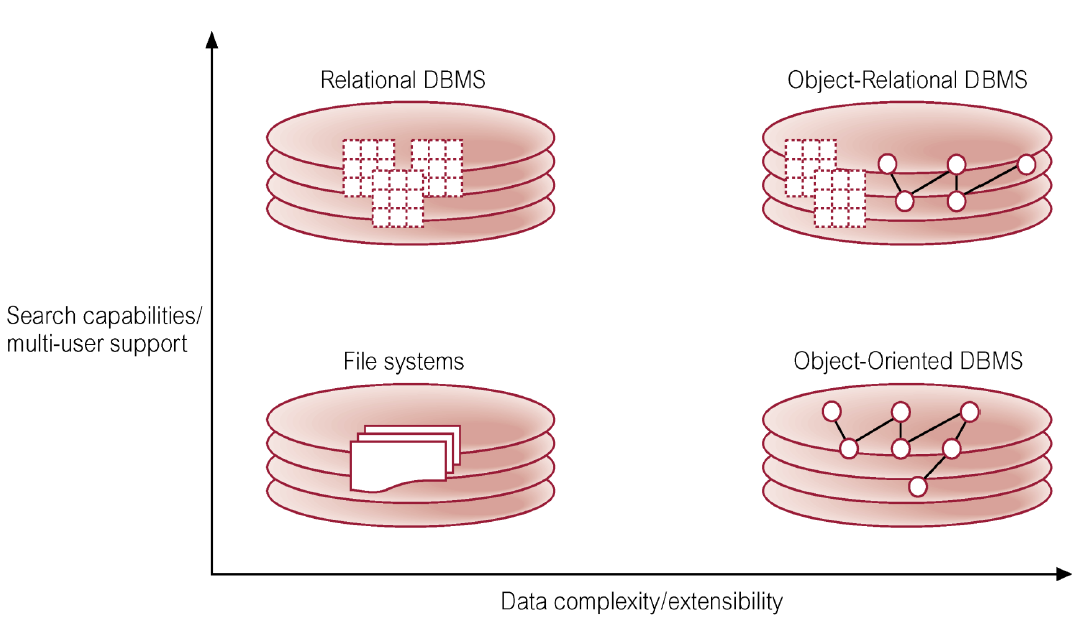
\includegraphics[width=.7\linewidth]{img/StonebreakersView.png}
\caption{Stonebreakers View}
\label{fig:StonebreakersView}
\end{figure}

\subsubsection{Voordelen van ORDBMS}
Oplossing voor de grote zwaktes van het relationeel model
\begin{itemize}
\item zwakke representatie van 'real-world' entiteiten
\item semantische overloading
\item zwakke ondersteuning voor integriteit en andere constraints
\item homogene data structuur
\item beperkte operaties
\item geen recursie
\item impedance mismatch
\item hergebruiken delen
\begin{itemize}
\item uitbreiden van de server functionaliteit om functionaliteit centraal uit te voeren
\item de centraal gedefinieerde functionaliteit kan nu gebruikt worden door alle applicaties
\end{itemize}
\item met als gevolg een hogere productiviteit
\item behoud van expertiseen kennisvan RDBMS
\item backwardscompatibility
\end{itemize}

\subsubsection{Nadelen van ORDBMS}
\begin{itemize}
\item complexiteit van het OR model: eenvoud en puurheid van het relationeel model gaat verloren
\item verhoogdekosten
\item enkel een klein deel van de applicaties kan gebruik maken van de object extensies
\item het is niet puur OO
\begin{itemize}
\item OO applicaties zijn niet zo data gecentreerd
\item in pure OO zijn objects first class citizens, geen extensies van het relationele model
\end{itemize}
\item SQL is te complex geworden
\end{itemize}


\subsubsection{Impedance Mismatch}
Er zijn verschillen tussen OO-model en relationeel model.

Dit probleem kan opgelost worden met OR-mapping of met User defined types.

\subsection{User Defined Types}
User defined types zijn abstracte types.
Deze types kunnen gebruikt worden als built-in type.

Er zijn twee soorten:
\begin{enumerate}
\item distinct types
\item structured types
\end{enumerate}

\subsubsection{Distinct types}
Een distinct type is gebaseerd op een basis type.
Het laat toe om onderscheid aan te brengen tussen anders gelijke basis types.

\subsubsection{Structured Types}
\textbf{Table Types}

Table types worden opgeslagen in de DB.
Deze types zijn tabellen.

Table variables bestaan slechts voor de duur van de batch.

\begin{itemize}
\item Voordelen:
	\begin{itemize}
	\item kortere en overzichtelijke code
	\item table type variabelen kunnen als parameters doorgegeven worden aan stored procedures en functions
	\end{itemize}
\end{itemize}

\textbf{Abstract Data Types}

In het algemeen bevat een abstract data type:
\begin{itemize}
\item definitie van de attributen
\item definitie van de routines (methodes)
\end{itemize}

Abstracte data types worden gebruikt om objecten op te slaan.

\subsubsection{Overerving}
Via \textsc{under} kunnen subtype/supertype verbanden gedefinieerd worden.

Multiple inheritance is niet mogelijk.

Het subtype erft de attributen en methodes van het supertype.
Het subtype kan uitgebreidt worden via definitie van nieuwe attributen en methodes.

Overloading van methodes is mogelijk.

Een supertype kan altijd door zijn subtype gesubstitueerd worden.

Men kan aan een \textsc{ADT} methodes toevoegen en deze implementeren in het \textsc{create type body} statement.

\textbf{NOT FINAL}: er kunnen nog subtypes gemaakt worden.

\textbf{FINAL}: er kunnen geen substypes gemaakt worden. (\textsc{default})

\subsection{Large Objects}
Een large object is een datatype die een grote hoeveelheid aan data kan vasthouden.

Er zijn verschillende soorten large objects:
\begin{itemize}
\item Binary Large OBject (BLOB)
\item Character Large OBject (CLOB)
\item National Character Large OBject (NCLOB)
\end{itemize}

De problemen met veel LOB's, die nu gebruikt worden in verschillende DBMS zijn:
\begin{itemize}
\item LOB's worden gezien als bytestreams
\item DBMS kan zelf niets aanvangen met LOB's
\item nadelig transfer van LOB'so p server naar client over het netwerk
\end{itemize}

\section{Transactiebeheer}
\subsection{Inleiding}
Een DBMS ondersteunt:
\begin{itemize}
\item transaction support
\item concurrency control service
\item recovery services
\end{itemize}

De bedoeling van transacties is dat de databank in een betrouwbare en consistentie toestand gehouden wordt.
\begin{itemize}
\item bij software/hardware failures
\item bij gelijktijdig gebruik door meerdere gebruikers
\end{itemize}

\subsection{Transacties}
Een transactie is een actie, of een opeenvolging van acties op een DB die 1 logisch geheel vormen.
\begin{itemize}
\item Een actie: lezen of wijzigen van de inhoud van de DB. Lees operaties berokkenen anderen nooit problemen. Je kan echter wel last hebben van anderen.
\item Een transactie wordt uitgevoerd door een gebruiker of door een programma.
\item Het is een logische eenheid van werk
\end{itemize}
\subsubsection{Resultaat van een transactie}
\begin{enumerate}
\item commited
	\begin{itemize}
	\item De transactie kent een succesvolle afloop
	\item De transactie commit en de DB heeft een consistente toestand bereikt.
	\end{itemize}
\item aborted
	\begin{itemize}
	\item De transactie is niet succesvol afgehandeld
	\item de transactie abort en de DB moet teruggebracht worden naar de consistente toestand waarin ze zich bevond voor de transactie werd gestart.
	
Dit gebeurt via \textsc{rollback} of \textsc{undo}
	\end{itemize}
\end{enumerate}

Een committed transaction kan nooit geaborted worden.

Een aborted transaction kan herstart worden.

\subsubsection{ACID Eigenschappen}
\textbf{Atomicity}: de opdrachten van een transactie worden als één ondeelbaar geheel beschouwd.
\begin{itemize}
\item alles of niets
\item DBMS verantwoordelijkheid: recovery subsystem
\end{itemize}

\textbf{Consistency}: een transactie brengt de DB van de een consistente toestand naar een andere consistente toestand.
\begin{itemize}
\item DBMS verantwoordelijkheid énprogramma verantwoordelijkheid
\end{itemize}

\textbf{Isolation}: transacties worden onafhankelijk van elkaar uitgevoerd.
\begin{itemize}
\item transacties mogen niet ongewenst interfereren met elkaar
\item transacties mogen geen uitkomsten aan andere transacties presenteren vóór de commit
\item DBMS verantwoordelijkheid: concurrency-controlsubsystem
\end{itemize}

\textbf{Durability}: na een COMMIT zijn de aangebrachte wijzigingen gegarandeerd permanent
\begin{itemize}
\item na een storing kunnen deze wijzigingen steeds worden gerecupereerd
\item DBMS verantwoordelijkheid: recovery subsystem
\end{itemize}

\subsubsection{Databank architectuur - Transaction support}
\begin{figure}[H]
\centering
  	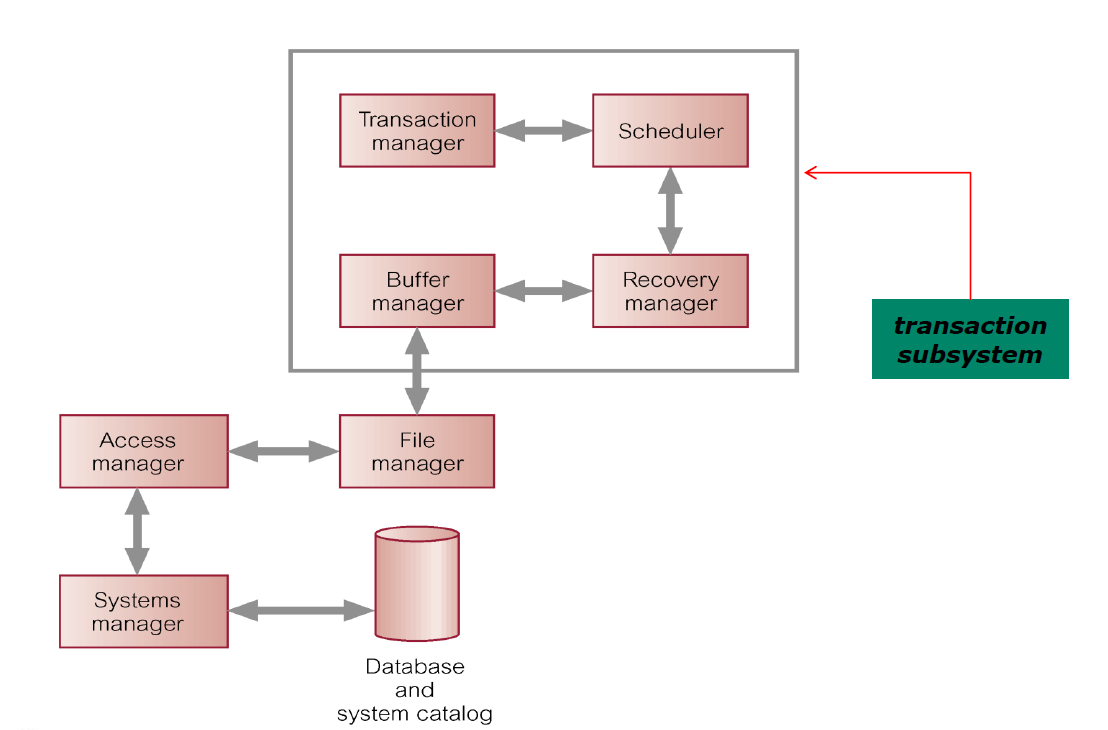
\includegraphics[width=.65\linewidth]{img/databankArchitectuur.png}
  	\caption{Databank architectuur - Transaction support}
  	\label{fig:DatabankArchitectuur}
\end{figure}

\begin{figure}[H]
\centering
  	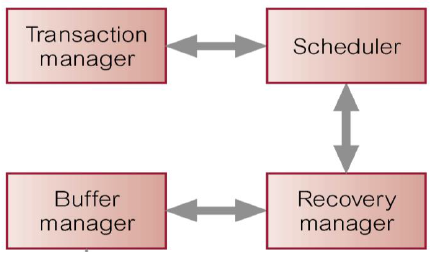
\includegraphics[width=.35\linewidth]{img/transactionSubsysteem.png}
  	\caption{Transactie subsysteem}
  	\label{fig:TransactieSubsysteem}
\end{figure}

\begin{itemize}
\item transaction manager
	\begin{itemize}
	\item coördineert transacties van programma's
	\end{itemize}
\item scheduler
	\begin{itemize}
	\item implementeert strategie voor concurrency control
	\item akalock manager bij een op locking gebaseerde strategie
	\item doel: concurrency maximaliseren zonder interferentie tussen verschillende transacties
	\end{itemize}
\item recovery manager
	\begin{itemize}
	\item bij failures brengt deze de db terug in consistente toestand (vóór de transactie gestart werd)	
	\end{itemize}
\item buffer manager
	\begin{itemize}
	\item verantwoordelijk voor efficiënte transfer van data tussen main memory en disk storage
	\end{itemize}
\end{itemize}

\subsection{Concurrency Control}
concurrency control is het beheer van gelijktijdige acties op de DB zonder dat ze interfereren met elkaar.

\subsubsection{Waarom?}
Concurrency Control voorkotm interferentie wanneer twee of meerdere transacties de databank gelijktijdig aanspreken, en minstens 1 transactie data wijzigt.

Hoewel twee transacties op zichzelf beschouwd correct kunnen zijn, kan het verweven van hun acties leiden tot een incorrect resultaat.

\subsubsection{Problemen bij concurrency control}
\textbf{Lost update}

Het lost update probleem treedt op wanneereen schijnbaar compleet succesvolle update van een transactie wordt overschreven door een andere transactie.

\textbf{Uncommitted Dependency}

Het uncommitted dependency (of dirty read) probleem treedt op wanneer een transactie de intermediaire resultaten van een andere, uncommitted transactie, kan zien.

Uncommited Dependency staat ook bekend als Dirty Read.

\textbf{Inconsistent Analysis}

Het inconsistent analysis probleem treedt op wanneer een transactie verschillende waarden uit de DB leest, terwijl een andere transactie bezig is sommige van deze waarden te veranderen.

Twee gerelateerde problemen aan de inconsistent analysis zijn:
\begin{enumerate}
\item non-repeatable read of fuzzy read
	\begin{itemize}
	\item Twee keer lezen van eenzelfde item levert twee verschillende waarden op.
	\end{itemize}
\item phantom read
	\begin{itemize}
	\item Een transactie leest een aantal records die voldoen aan een bepaalde voorwaarde.
	\item De transactie herhaalt dit later maar merkt nu dat er ondertussen andere records zijn bijgekomen via een andere transactie.
	\end{itemize}
\end{enumerate}

\subsubsection{Serializability en recovery}
\textbf{Schedule}

een schedule is een sequentie van acties van een aantal concurrente transacties die de volgorde van de acties van de individuele transacties respecteert.

\textbf{Recoverability}

De databank zelf schedules laten opstellen die zonder interferentie problemen concurrent kunnen worden uitgevoerd.
\begin{itemize}
\item ze garanderen de consistencyen isolationeigenschap van transacties
\item dit is in de veronderstelling dat geen enkele van de transacties in de schedule faalt
\end{itemize}
recoverability:
\begin{itemize}
\item wanneer een transactie faalt moeten we de effecten ongedaan kunnen maken.
	\begin{itemize}
	\item atomiciteitvan transacties
	\end{itemize}
\item wanneer een transactie commit zijn de veranderingen permanent
	\begin{itemize}
	\item durability eigenschap van transacties
	\end{itemize}
\end{itemize}

\subsubsection{Locking}
Locking is een methode gebruikt om concurrente toegang tot data te beheren.

Wanneer een transactie toegang heeft tot de DB kan er via een lock voor gezorgd worden dat andere transacties toegang tot de DB geweigerd worden om zo incorrecte resultaten te voorkomen.

Locking is de meest gebruikte manier om de consistentie te garanderen.

\textbf{Basisregels voor locking}

Een transactie kan een data item lezen of schrijven enkel en alleen als het een lock heeft verworven voor dat data element, en het bovendien deze lock nog niet heeft vrijgegeven.

Als een transactie een lock op een data item verwerft, dan moet het later ook die lock terug vrijgeven.

\textbf{Soorten locks}

Shared locks (S-Locks):
\begin{itemize}
\item een transactie met een shared lock op een data item kan dat data item lezenmaar niet wijzigen
\item meerdere transacties kunnen gelijktijdig een shared lock op eenzelfde data item bezitten
\end{itemize}
Exclusive locks (X-Locks):
\begin{itemize}
\item een transactie met een exclusive lock op een data item kan dat data item lezen en wijzigen
\item op elk ogenblik kan hoogstens 1 transactie een exclusive lock op een data item hebben
\end{itemize}
\subsubsection{Deadlock}
Een impasse die kan ontstaan wanneer twee of meerdere transacties elk wachten op het vrijgeven van locks die de andere transactie heeft.

Het oplossen van een deadlock gaat meestal als volgt:
abort en restart 1 of meerdere transacties.

\textbf{Timeouts}

Een transactie die een lock aanvraagt wacht voor een bepaalde vooraf gedefinieerde tijdop die lock.

Indien lock niet toegekend tijdens dit interval
\begin{itemize}
\item Assumptie dat er een deadlock is.
	\begin{itemize}
	\item hoewel dit niet noodzakelijk zo is\dots
	\end{itemize}
\item Aborten restartvan de transactie.
\end{itemize}

\textbf{Deadlock Prevention}

\begin{itemize}
\item Gebruik makend van transaction time-stamps
	\begin{itemize}
	\item time-stampvoor deadlock detection
	\end{itemize} 
\item T wacht op locks die U vast heeft
	\begin{itemize}
	\item wait-diealgoritme
		\begin{itemize}
		\item als T ouder is dan U dan zal T wachten
		\item in ander geval 'sterft' T
			\begin{itemize}
			\item abort/restart met dezelfde timestamp
			\end{itemize}
		\end{itemize}
	\item wound-waitalgoritme
		\begin{itemize}
		\item als T ouder is dan U dan zal het U 'verwonden'
			\begin{itemize}
			\item meestal betekent dit een abort/restart van U
			\end{itemize}
		\item in andere geval zal T wachten
		\end{itemize}
	\end{itemize}
\end{itemize}

\textbf{Deadlock Detection en Recovery}

Detection:
\begin{itemize}
\item Gebruik makend van een wait-for graph met transactie afhankelijkheden
\item Wanneer de wait-for graph een lus bevat is er een deadlock
\item Op regelmatige tijdstippen wordt deze graph getest op lussen
\end{itemize}
Recovery:
\begin{itemize}
\item 1 of meerdere transacties worden ge-abort
\item Problemen:
	\begin{itemize}
	\item Victim Selection
		\begin{itemize}
		\item abort die transactie waarvoor de abort een 'minimale kost' met zich meebrengt.
		\item enkele parameters die kunnen gebruikt worden:
			\begin{itemize}
			\item tijd dat de transactie al aan het runnen was
			\item aantal data items dat reeds werd gewijzigd door de transactie
			\item aantal data items die nog moeten worden gewijzigd door de transactie
			\end{itemize}
		\end{itemize}
	\item hoe ver moet een transactie een rollback doen
		\begin{itemize}
		\item dit is niet noodzakelijk de volledige transactie
		\end{itemize}
	\item voorkomen van starvation
		\begin{itemize}
		\item komt voor wanneer steeds dezelfde transactie als victim wordt geselecteerd.
			\begin{itemize}
			\item teller bijhouden
			\end{itemize}
		\end{itemize}
	\end{itemize}
\end{itemize}
\subsection{Transacties in SQL-server}
Impliciete transacties:
\begin{itemize}
\item insert, update, delete
\item elke transact sql-opdracht
\end{itemize}

Expliciete transacties:
\begin{itemize}
\item zelf aangeven waar transactie begint, wanneer de transactie kan afgesloten worden, of hoe je op je stappen terugkeert om fouten op te vangen.
	\begin{itemize}
	\item BEGIN TRANSACTION
	\item COMMIT TRANSACTION
	\item ROLLBACK TRANSACTION
	\end{itemize}
\end{itemize}

\subsubsection{Isolation levels}
Bepalen het gedrag van concurrent users die data lezen of schrijven.
\begin{itemize}
\item Reader: statement dat data leest, m.b.v. een shared lock
\item Writer: statement dat data schrijft, m.b.v. een exclusive lock
\end{itemize}
Writers kun je niet beïnvloeden voor wat betreft de locks die ze nemen en de duur van de locks.

Readers kun je wel expliciet beïnvloeden, hierdoor heb je impliciet invloed op het gedrag van de writers.

Isolation level = setting op sessie-niveau of query-niveau.

\subsubsection{Isolation levels in SQL-server}

\begin{enumerate}
\item read uncommitted
\item read committed (default)
\item repeatable read
\item serializable
\end{enumerate}

Hoe hoger het nummer hoe minder beperkingen, hoe lager het nummer hoe meer afscherming en dus meer hinder voor andere sql statements.

\textbf{Read uncommitted}
\begin{itemize}
\item laagste isolatieniveau
\item reader vraagt geen shared lock
\item reader nooit in conflict met writer, die exclusieve lock heeft
\item reader lees incommited data (=dirty read)
\end{itemize}

\textbf{Read committed}
\begin{itemize}
\item default isolation level
\item laagste niveau dat dirty reads verhindert
\item reader leest enkel committed data
\item reader vraagt hiervoor een shared lock
\item als bij deze vraag een writer een exclusive lock heeft, moet de reader wachten op shared lock
\item reader houdt shared lock tot de data verkregen is, niet tot einde van zijn transactie
	\begin{itemize}
	\item nogmaals lezen van de tata in dezelfde transactie kan een ander resultaat opleveren
	
	= non-repeatable reads of inconsistent analysis
	\item acceptabel voor veel toepassingen
	\end{itemize}
\end{itemize}

\textbf{Repeatable read}
\begin{itemize}
\item reader vraagt shared lock en houdt deze tot het einde van de transactie.
\item andere transactie kan geen exclusive lock verkrijgen tot einde van de transactie van de reader
\item repeatable read = consistent analysis
\item vermijd ook \textit{lost update} door bij het begin van de transactie shared lock te nemen
\end{itemize}

\textbf{Serializable}
\begin{itemize}
\item repeatable read lockt enkel rijen gevonden door de eerste SELECT.
\item zelfde SELECT in dezelfde transactie kan nieuwe rijen geven = \textit{phantoms}
\item Serializable vermijdt deze phantoms
\item lockt alle keys die beantwoorden aan de WHERE-clause, ook toekomstige
\end{itemize}

\subsubsection{Isolation levels: Sessie niveau}
\begin{lstlisting}[language=sql, breaklines=true]
SET TRANSACTION ISOLATION LEVEL [isolationlevel]
\end{lstlisting}

\subsubsection{Isolation levels: Query niveau}
\begin{lstlisting}[language=sql, breaklines=true]
SELECT * FROM ORDERS WITH (NOLOCK);
of
SELECT * FROM ORDERS WITH (READUNCOMMITTED);
\end{lstlisting}
Dit vermijdt dat langlopende ad-hoc query's op productie-systeem updates in andere transacties laten wachten bij READ COMMITTED en hoger.

\subsection{Recovery}
Recovery is het proces waarbij een DB wordt teruggebracht naar een correcte toestand wanneer er zich een failure voordoet.

\subsubsection{Media}
\begin{itemize}
\item Main memory
	\begin{itemize}
	\item random acces
	\item online
	\item vluchtig
	\item onbetrouwbaar
	\item duur
	\item zeer snel
	\end{itemize}
\item Magnetic disc
	\begin{itemize}
	\item random acces
	\item online
	\item niet vluchtig
	\item onbetrouwbaar
	\item minder duur
	\item snel
	\end{itemize}
\item Tape (casette): voornamelijk backup's en zaken die weinig gebruikt worden
	\begin{itemize}
	\item sequentieel
	\item online of offline
	\item niet vluchtig
	\item zeer betrouwbaar
	\item goedkoop
	\item traag
	\end{itemize}
\item Optical disc
	\begin{itemize}
	\item random acces
	\item online of offline
	\item niet vluchtig
	\item zeer betrouwbaar
	\item zeer goedkoop
	\item traag
	\end{itemize}
\end{itemize}
Stabiele opslag: replicatie op verschillende plaatsen

Mirroring: quasi tegelijk naar meerdere locaties gegevens wegschrijven

Virtuele tapedrives: gesimuleerde tapedrives op een disk en pas als er op de de virtuele tapedrive geen plaats meer is op de virtuele tape naar een reële tape wegschrijven.
Dit zorgt voor perfomatie winst, omdat de write acties korter zijn naar de disk en omdat de tapes altijd volledig vol zijn.
Er zijn dus nooit tapes die niet volledig gevuld zijn met data.

\subsubsection{Soorten failures}
System crash
\begin{itemize}
\item hardware of software errors
\item verlies van gegevens in main memory
\end{itemize}
Media failure
\begin{itemize}
\item vb. disk head crasht
\item verlies van gegevens in secondary storage
\end{itemize}
Software error in applicaties
\begin{itemize}
\item vb. logische fout die transacties doet falen
\end{itemize}
Natuurlijke rampen
\begin{itemize}
\item vb. brand, aardbeving
\end{itemize}
Slordigheid
\begin{itemize}
\item vb. onopzettelijk wissen van gegevens door de gebruiker of DB admin
\end{itemize}
Sabotage
\begin{itemize}
\item vb. opzettelijk wissen of corrupteren van gegevens of infrastructuur
\end{itemize}

\subsubsection{Transactions en recovery}
De eenheid voor recovery is een transactie.

De recovery manager staat voor:
\begin{itemize}
\item atomiciteit (\textbf{A}CID)
\item duurzaamheid (ACI\textbf{D})
\end{itemize}
De moeilijkheid hierbij is dat het schrijven naar een databank niet atomaire is.
Een transactie kan committen zonder dat alle effecten al (permanent) in de DB geregistreerd zijn.

\subsubsection{Undo en Redo}
Enkel bij een flush van de buffer is de data permanent.
\begin{itemize}
\item \textbf{Flushing}: data overhevelen van primary storage naar disk storage
\end{itemize}
Expliciete flush
\begin{itemize}
\item force writing
\item dit gebeurt via een commando, vb. commit
\end{itemize}
Impleciete flush
\begin{itemize}
\item wanneer de buffers vol zijn
\end{itemize}
Als er een failure is tussen het schrijven naar de buffer en de flushing dan:
\begin{itemize}
\item Transactie was reeds gecommit
	\begin{itemize}
	\item durability: redo de wijzigingen
	\item aka roll forward
	\end{itemize}
\item Transactie was nog niet gecommit
	\begin{itemize}
	\item atomicity: undo de wijzigingen
		\begin{itemize}
		\item partiële undo: undo van 1 transactie
		\item globale undo: undo van alle actieve transacties
		\end{itemize}
	\item aka rollback
	\end{itemize}
\end{itemize}
\subsubsection{Buffer management}
buffer management omvat het beheer van transfer van buffers tussen main memory en disk.

Praktisch:
\begin{itemize}
\item inlezen tot buffer vol
\item replacement strategie voor force-write
	\begin{itemize}
	\item FIFO: first in first out
	\item LRU: least recently used
	\end{itemize}
\end{itemize}

\subsubsection{Recovery faciliteiten}
Het DBMS beidt de volgende diensten aan:
\begin{itemize}
\item back-up mechanisme
	\begin{itemize}
	\item periodische back-ups van de DB, dit gebeurt automatisch zonder dat de systemen moeten stoppen en de kopieën worden bewaard op offline storage.
	\item compleet of incrementeel
	\end{itemize}
\item logging mogelijkheden
	\begin{itemize}
	\item op de hoogte blijven van de huidige toestand van transacties 	en db wijzigingen
	\item de log bevat mogelijks: transaction id, type of log record, id van de gewijzigde data, before image, after-image
	\item log wordt ook gebruikt voor performance monitoring en auditing
	\item log is belangrijk wordt in 2 of 3 voud bijgehouden, ook offline
	\item log moet snel toegankelijk zijn: minor failures moeten direct opgelost worden $\rightarrow$ liefst ook op online storage
	\end{itemize}
\item checkpoint mogelijkheden
	\begin{itemize}
	\item om lopende wijzigingen in de db permanent te maken
	\end{itemize}
\item recovery manager
	\begin{itemize}
	\item om de db in een consistente toestand te brengen na een failure
	\end{itemize}
\end{itemize}

\subsubsection{Checkpointing}
Een checkpoint is een synchronisatiepunt tussen de databank en de log,
op dit punt worden alle buffers ge-flushed.

Checkpoints worden voorzien op vooraf ingestelde intervallen.

Een checkpoint omvat:
\begin{itemize}
\item alle log records in main memory wegschrijven naar disk
\item de gewijzigde delen van de buffers wegschrijven naar disk
\item een checkpoint record in de log registreren
	\begin{itemize}
	\item dit record bevat id van alle transacties die actief zijn op het moment van checkpointing
	\end{itemize}
\end{itemize}

\subsubsection{Recovery technieken}
Soort recovery procedure die gevolgd wordt hangt af van de ernst van het probleem.
\begin{itemize}
\item serieuze problemen
	\begin{itemize}
	\item backup restoren
	\item wijzigingen van committed transacties (sedert de backup) die verloren gingen, herstellen adhvde log
	\end{itemize}
\item problemen van inconsistentie
	\begin{itemize}
	\item kan zonder backup
	\item undo/redo adhvde log'sbeforeen afterimages
	\end{itemize}
\end{itemize}

\subsubsection{Deferred update}
Bij een deferred recovery protocol worden wijzigingen van een transactie niet weggeschreven naar de dbzolang de transactie niet het commit-punt bereikt.
\begin{enumerate}
\item start van de transactie
	\begin{itemize}
	\item registreert transaction start in de log
	\end{itemize}
\item bij een write actie
	\begin{itemize}
	\item registreert dit in de log: enkel after-image, geen before-image nodig
	\item registreert dit niet in de DB
	\end{itemize}
\item commit van de transactie
	\begin{itemize}
	\item registreert transaction commit in de log
	\item schrijf alle log records weg naar disk (flush de log vóór de volgende stap!)
	\item commit, update de DB adhv de log records
	\end{itemize}
\item abort van de transactie
	\begin{itemize}
	\item negeer de log records, schrijf niets naar disk
	\end{itemize}
\end{enumerate}

\subsubsection{Immediate update}
bij een immediateupdate recovery protocol worden wijzigingen van een transactie direct weggeschreven naar de DB.
\begin{enumerate}
\item start van de transactie
	\begin{itemize}
	\item registreer transaction start record in log
	\end{itemize}
\item bij een write actie
	\begin{itemize}
	\item schrijf het log-record naar disk: het log-recordbevat before-image en after-image
	\item bij flush van de buffers wordt de wijziging naar de DB geschreven
	\end{itemize}
\item commit van de transactie
	\begin{itemize}
	\item schrijf een transaction commit log record naar disk
	\end{itemize}
\item abort van de transactie
	\begin{itemize}
	\item gebruik before-images voor undo
	\end{itemize}
\end{enumerate}
\end{document}